\newpage
\section*{CHAPTER 4. EXPERIMENTAL RESULTS}
\phantomsection\addcontentsline{toc}{section}{\numberline{}CHAPTER 4. EXPERIMENTAL RESULTS}
\setcounter{section}{4}
\setcounter{subsection}{0}
\setcounter{subsubsection}{0}
\setcounter{paragraph}{0}
\setcounter{figure}{0}
\setcounter{table}{0}

Chapter 4 presents the experimental procedure and evaluation results of the proposed quantized HiFiC GAN accelerator. Following an evaluation-oriented structure, this chapter first describes the accuracy evaluation environment, then reports FPGA resource utilization, analyzes performance, compares the hardware-oriented implementation with the software reference, and finally summarizes the main observations.

%%%%%%%%%%%%%%%%%%%%%%%%%%%%%%%%%%%%%%%%%%%%%%%%%%%%%%%%%%%%%%%%%%%%%%%%%%%%%%%%%%%%%%%%%%%%%%%%%%%%
\subsection{Accuracy Evaluation}

The first objective of the evaluation is to verify that the hardware-oriented implementation preserves the functional behavior of the HiFiC inference pipeline. Since the proposed accelerator targets the ResBlock computation inside the generator, the verification process compares the HLS/FPGA-oriented output with the Python reference model using the same input feature data and model parameters.

\subsubsection{Verification Environment}

Figure~\ref{fig:system_architecture} illustrates the verification and deployment environment used in this project. The system follows a hardware--software co-design approach on the ZCU104 platform. The Processing System (PS) is responsible for software control, memory management, and accelerator invocation, while the Programmable Logic (PL) implements the custom ResBlock accelerator.

\begin{figure}[H]
    \centering
    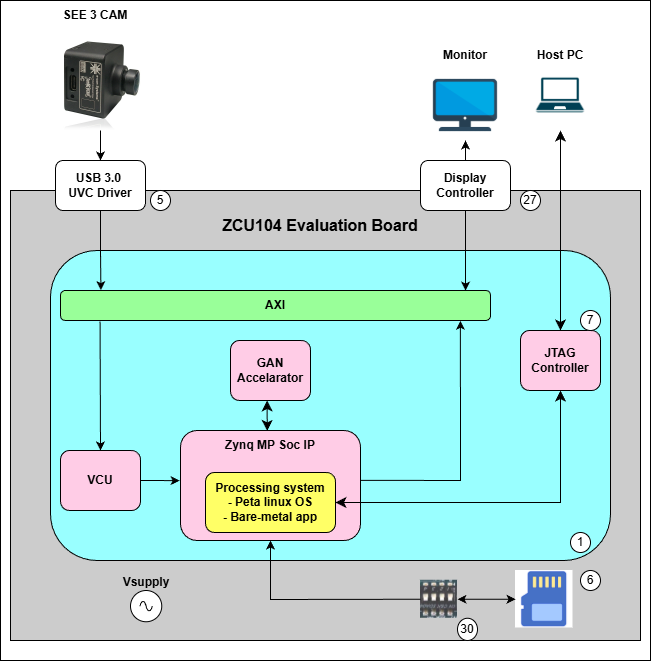
\includegraphics[width=1\linewidth]{Images/System Architecture.png}
    \caption{Verification and deployment environment on the ZCU104 platform}
    \label{fig:system_architecture}
\end{figure}

The software reference is executed in Python to generate golden outputs for comparison. The same input tensors, weights, and normalization parameters are then used by the HLS C/C++ implementation. During simulation, the output of the HLS model is compared with the Python reference to verify numerical consistency. After successful HLS verification, the generated IP core is integrated into the Vivado block design shown in Figure~\ref{fig:vivado_block_design}.

\begin{figure}[H]
    \centering
    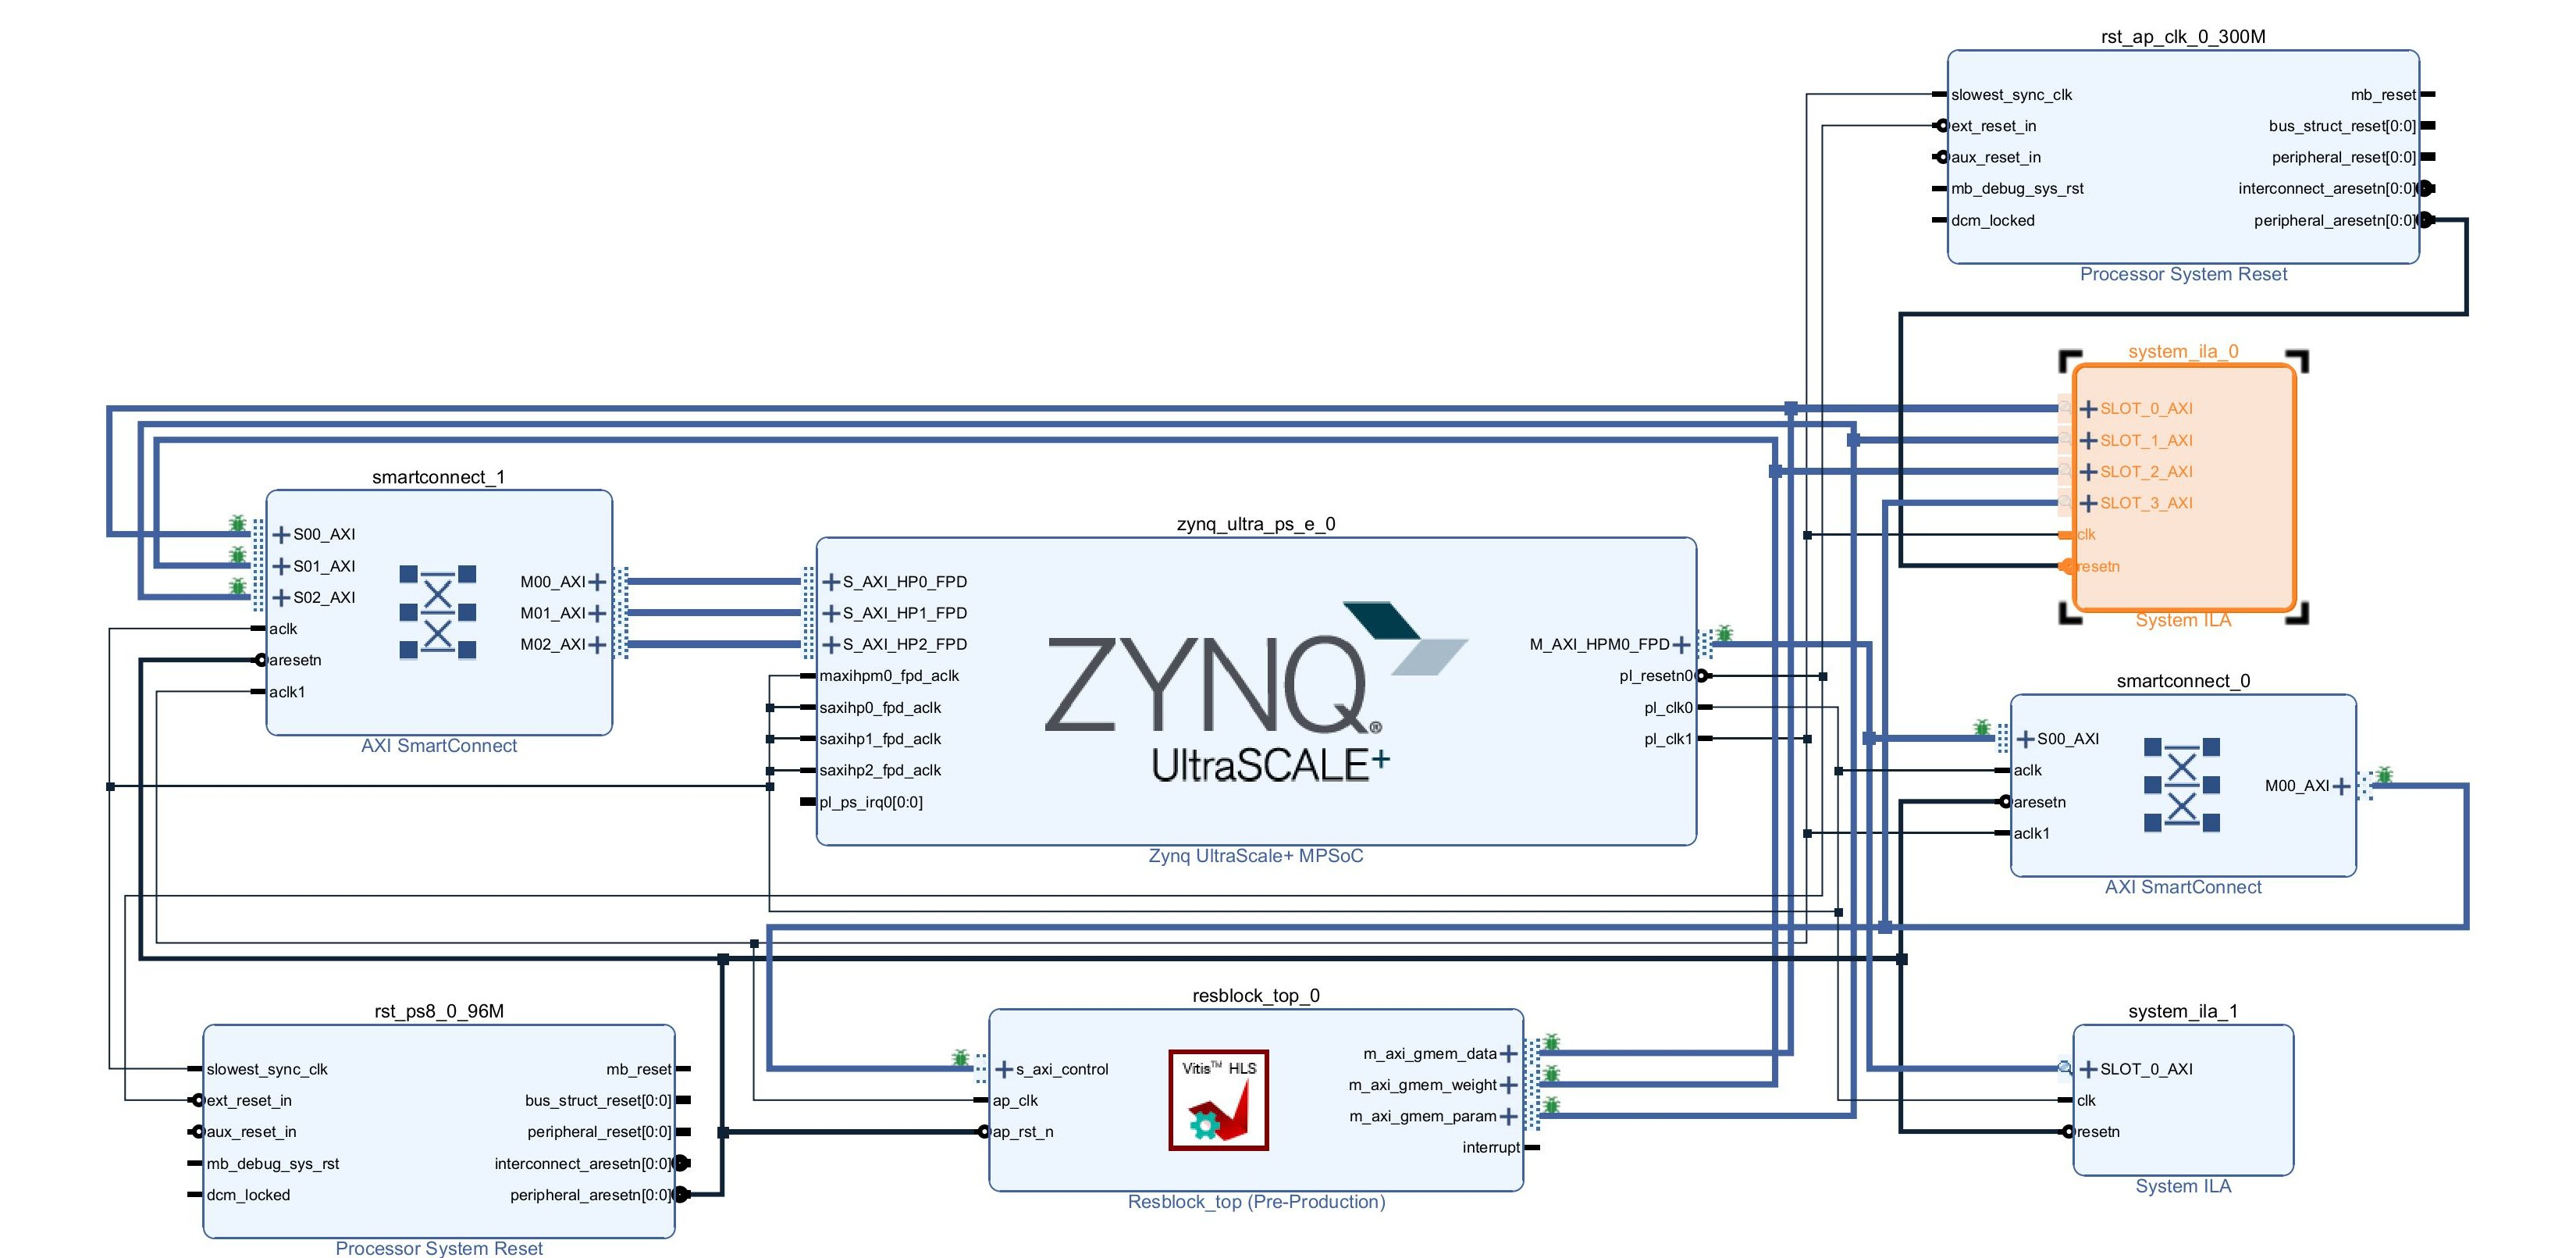
\includegraphics[width=1\linewidth]{Images/block_design.jpg}
    \caption{Vivado block design of the proposed accelerator system}
    \label{fig:vivado_block_design}
\end{figure}

The target board used for implementation is the Zynq\texttrademark{} UltraScale+\texttrademark{} MPSoC ZCU104, shown in Figure~\ref{fig:ZCU}. The most relevant components for this project are summarized in Table~\ref{tab:zcu104_components}. These components provide the processing system, programmable logic, external memory, SD-card boot interface, and display/output connections required for testing the accelerator.

\begin{figure}[H]
    \centering
    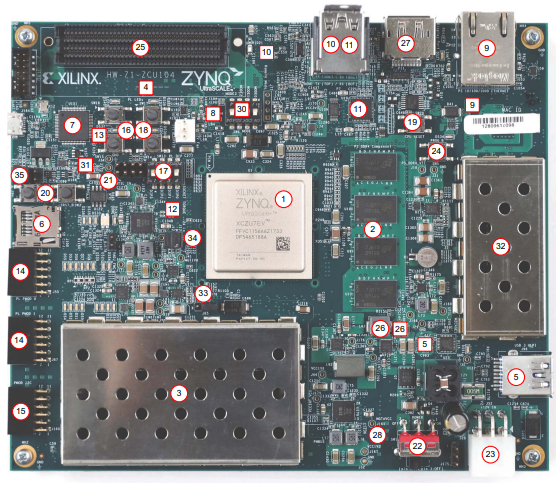
\includegraphics[width=0.9\linewidth]{Images/ZCU.png}
    \caption{Zynq\texttrademark{} UltraScale+\texttrademark{} MPSoC ZCU104 evaluation board}
    \label{fig:ZCU}
\end{figure}

\begin{table}[H]
    \centering
    \caption{Relevant ZCU104 components for accelerator evaluation}
    \label{tab:zcu104_components}
    \begin{tabular}{|c|l|}
        \hline
        \textbf{No.} & \textbf{Component} \\
        \hline
        1 & Zynq UltraScale+ XCZU7EV MPSoC \\
        \hline
        3 & PL-side SODIMM DDR4 memory \\
        \hline
        5 & USB 3.0 transceiver and USB 2.0 ULPI PHY \\
        \hline
        6 & SD-card interface connector \\
        \hline
        7 & Programmable Logic JTAG \\
        \hline
        27 & DisplayPort connector \\
        \hline
    \end{tabular}
\end{table}

The verification flow consists of four main steps. First, the Python reference model produces the expected reconstructed output or intermediate feature output. Second, the HLS C/C++ model processes the same input data using the hardware-oriented implementation. Third, the two outputs are compared using objective image-quality metrics. Finally, after synthesis and implementation, the accelerator is controlled from Vitis on the ZCU104 platform to measure board-level behavior.

\subsubsection{Test Images and Evaluation Metrics}

The evaluation uses representative RGB images resized to $256 \times 256$, consistent with the input size used throughout this thesis. The reconstructed images are evaluated using image-quality metrics introduced in Chapter~2, including Peak Signal-to-Noise Ratio (PSNR), Structural Similarity Index Measure (SSIM), and Mean Squared Error (MSE). These metrics are suitable for checking whether the quantized hardware-oriented implementation remains close to the software reference.

Figure~\ref{fig:chapter4_psnr_comparison} shows the PSNR comparison between the Python reference model and the HLS simulation model over 100 test images. The similarity of the two curves indicates that the HLS implementation follows the numerical behavior of the reference model closely enough for FPGA deployment.

\begin{figure}[H]
    \centering
    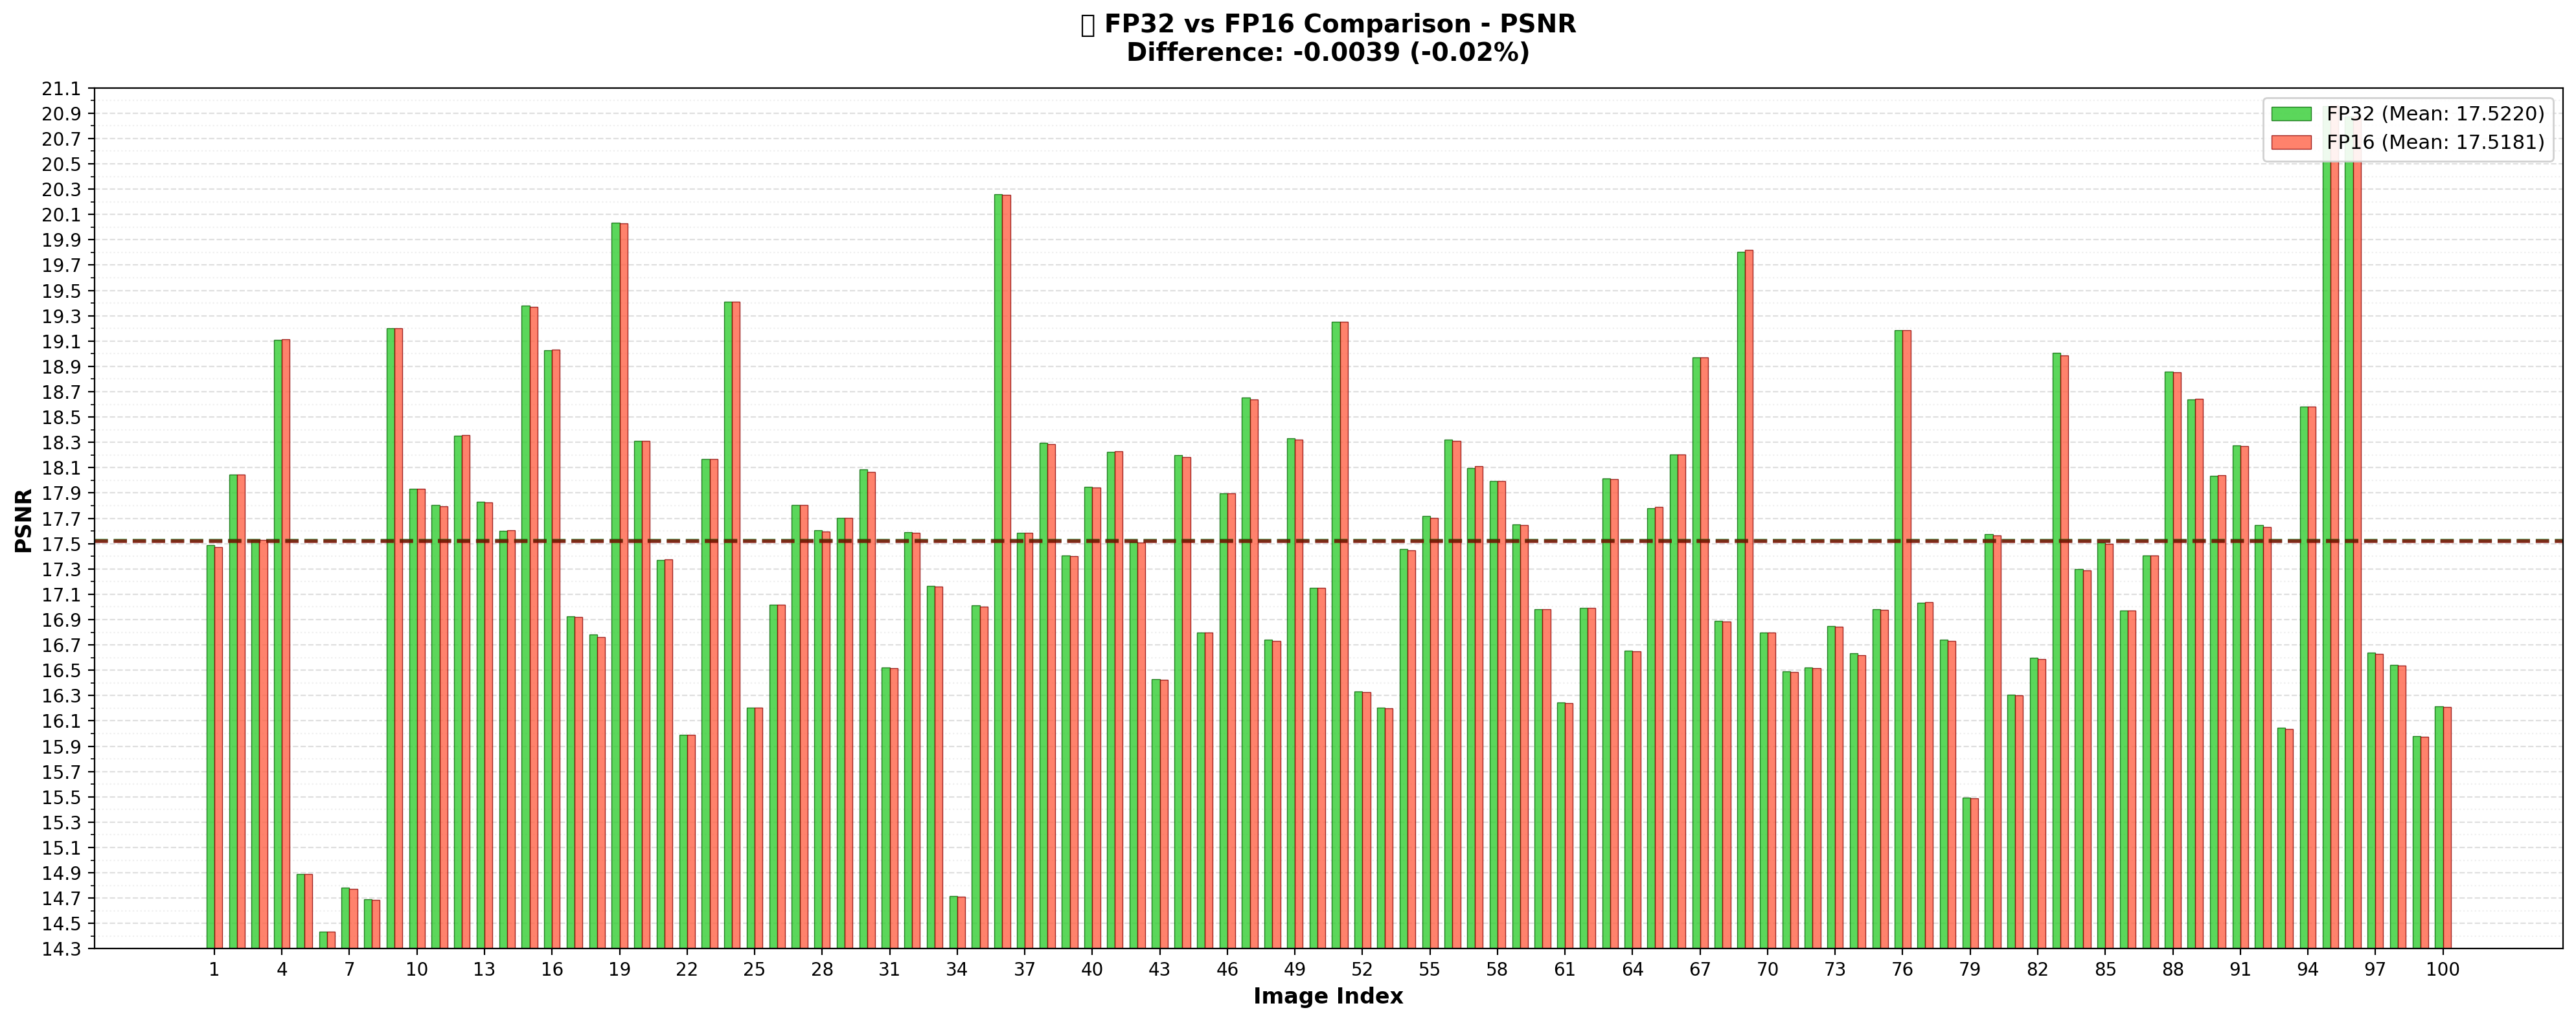
\includegraphics[width=1\linewidth]{Images/comparison_psnr_sidebyside.png}
    \caption{PSNR comparison between the Python reference model and the quantized HLS simulation model}
    \label{fig:chapter4_psnr_comparison}
\end{figure}

Overall, the accuracy evaluation confirms that the hardware-oriented ResBlock implementation preserves the main reconstruction behavior of the HiFiC generator. Small numerical differences are expected because the accelerator uses a mixed-precision data path, but the observed quality trend remains close to the Python reference.

%%%%%%%%%%%%%%%%%%%%%%%%%%%%%%%%%%%%%%%%%%%%%%%%%%%%%%%%%%%%%%%%%%%%%%%%%%%%%%%%%%%%%%%%%%%%%%%%%%%%
\subsection{Resource Utilization and Power Measurement}

After functional verification, the accelerator was synthesized and implemented on the ZCU104 FPGA platform to evaluate resource utilization. The implementation result reflects the cost of mapping the quantized ResBlock computation, local buffering, AXI-based data movement, and control logic into the Programmable Logic (PL). The target clock frequency is 300~MHz.

The hardware utilization report is summarized in Table~\ref{tab:hific_generator_utilization}. The implemented accelerator uses 182,374 LUTs, corresponding to 79\% of the available LUT resources, and 175,744 FFs, corresponding to 38\% of the available flip-flop resources. For on-chip storage, the design consumes 601 BRAM 18Kb blocks, or 96\% of the available BRAM resources, together with 68 URAM blocks, or 70\% of the available URAM resources. The arithmetic datapath uses 1,614 DSP slices, corresponding to 93\% of the available DSP resources.

\begin{table}[H]
    \centering
    \caption{Hardware resource utilization of the HiFiC generator ResBlock accelerator}
    \label{tab:hific_generator_utilization}
    \begin{tabular}{|l|c|}
        \hline
        \textbf{Resource} & \textbf{ResBlock Accelerator} \\
        \hline
        LUTs & 182,374 (79\%) \\
        \hline
        FFs & 175,744 (38\%) \\
        \hline
        BRAMs (18Kb Block) & 601 (96\%) \\
        \hline
        URAMs & 68 (70\%) \\
        \hline
        DSPs & 1,614 (93\%) \\
        \hline
        Frequency (MHz) & 300 \\
        \hline
    \end{tabular}
\end{table}

The utilization results show that the proposed accelerator is both computation-intensive and memory-intensive. DSP utilization is high because convolution dominates the ResBlock workload and requires a large number of multiply--accumulate operations. BRAM and URAM utilization are also high because intermediate feature maps, line buffers, weights, and partial results must be stored locally to reduce external DDR access and sustain the pipelined datapath.

Power measurement is evaluated as part of board-level deployment. In this design, the main contributors to dynamic power are expected to be DSP activity, BRAM/URAM access, AXI memory transfers, and clocked control logic. Therefore, reducing unnecessary memory movement and improving data reuse are important not only for performance but also for power efficiency.

%%%%%%%%%%%%%%%%%%%%%%%%%%%%%%%%%%%%%%%%%%%%%%%%%%%%%%%%%%%%%%%%%%%%%%%%%%%%%%%%%%%%%%%%%%%%%%%%%%%%
\subsection{Performance Evaluation}

In addition to resource utilization, several performance metrics are used to evaluate the effectiveness of the proposed accelerator. These metrics include operating frequency, throughput, accelerated block, numerical precision, and speedup compared with the software-only baseline.

Table~\ref{tab:performance_evaluation} summarizes the main performance results. The accelerator operates at 300~MHz and targets the ResBlock workload inside the HiFiC generator. The measured throughput is 33.2 GOPS. Based on the board-level Vitis application, the FPGA implementation achieves an approximately five-times speedup compared with the software-only execution path.

\begin{table}[H]
    \centering
    \caption{Performance evaluation of the proposed accelerator}
    \label{tab:performance_evaluation}
    \begin{tabular}{|l|c|}
        \hline
        \textbf{Metric} & \textbf{Result} \\
        \hline
        FPGA platform & ZCU104 \\
        \hline
        Frequency & 300~MHz \\
        \hline
        Accelerated block & HiFiC generator ResBlock \\
        \hline
        Precision & Mixed FP16 \\
        \hline
        Throughput & 33.2~GOPS \\
        \hline
        Speedup over software & Approximately $5\times$ \\
        \hline
    \end{tabular}
\end{table}

The performance result shows that the accelerator benefits from parallel DSP computation and local on-chip buffering. The ResBlock structure is suitable for FPGA acceleration because its convolution windows, channel accumulation, and residual operations are regular and can be pipelined. However, the high BRAM, URAM, and DSP utilization indicates that further performance scaling must be balanced carefully against the remaining device resources.

%%%%%%%%%%%%%%%%%%%%%%%%%%%%%%%%%%%%%%%%%%%%%%%%%%%%%%%%%%%%%%%%%%%%%%%%%%%%%%%%%%%%%%%%%%%%%%%%%%%%
\subsection{Comparison}

Table~\ref{tab:implementation_comparison} compares the main evaluation stages used in this thesis. The Python model serves as the golden reference, the HLS simulation verifies the hardware-oriented C/C++ design, and the FPGA implementation evaluates the accelerator on the ZCU104 platform.

\begin{table}[H]
    \centering
    \caption{Comparison between software reference, HLS simulation, and FPGA implementation}
    \label{tab:implementation_comparison}
    \resizebox{\textwidth}{!}{%
    \begin{tabular}{|l|c|c|c|}
        \hline
        \textbf{Evaluation Stage} & \textbf{Platform} & \textbf{Purpose} & \textbf{Main Observation} \\
        \hline
        Python reference model & CPU/GPU software & Golden output generation & Provides reference PSNR and reconstructed output. \\
        \hline
        HLS simulation model & Vitis HLS C/C++ simulation & Functional verification & Produces PSNR trend close to the Python reference. \\
        \hline
        FPGA accelerator & ZCU104 PL + PS & Hardware performance evaluation & Achieves approximately $5\times$ speedup over software-only execution. \\
        \hline
    \end{tabular}%
    }
\end{table}

The comparison indicates that the proposed workflow preserves correctness while moving the most computationally demanding workload from software to FPGA hardware. The HLS simulation validates the arithmetic behavior before hardware synthesis, while the ZCU104 implementation demonstrates the benefit of dedicated parallel computation for the ResBlock workload.

%%%%%%%%%%%%%%%%%%%%%%%%%%%%%%%%%%%%%%%%%%%%%%%%%%%%%%%%%%%%%%%%%%%%%%%%%%%%%%%%%%%%%%%%%%%%%%%%%%%%
\subsection{Chapter Conclusion}

Chapter 4 presented the experimental results of the proposed quantized HiFiC GAN accelerator. The accuracy evaluation compared the HLS simulation output with the Python reference model using PSNR over 100 test images. The resource utilization report showed that the design uses a large portion of the available DSP, BRAM, and URAM resources, which is expected for a highly parallel ResBlock accelerator. The performance evaluation demonstrated an operating frequency of 300~MHz, a throughput of 33.2~GOPS, and an approximately five-times speedup over the software-only baseline.

Overall, the results confirm that the proposed hardware--software co-design is suitable for accelerating the dominant ResBlock workload in the HiFiC generator. The next chapter further reports final verification results and discusses the implementation behavior on the ZCU104 platform.
